\documentclass{mirea}

\institution{Институт искусственного интеллекта}
\faculty    {Кафедра общей информатики}
\worktype   {ОТЧЕТ \\ ПО ПРАКТИЧЕСКОЙ РАБОТЕ №10}
\workname   {Изучение работы триггеров}
\subject    {ИНФОРМАТИКА}
\author     {Краснов Н.O.}
\examiner   {Павлова Е.С.}

\usepackage{tikz-timing}
\usepackage{float}

\begin{document}
	
\chapter{ПОСТАНОВКА ЗАДАЧИ}
	Изучить на практике работу разного вида триггеров.
	
\chapter{ПРОЕКТИРОВАНИЕ И РЕАЛИЗАЦИЯ}
\section{Одноступенчатый асинхронный RS-триггер на элементах <<И-НЕ>>}
	Таблица переходов триггера (табл. \ref{table:1stepAsyncRSNAND}) и его функциональная схема (рис. \ref{fig:1stepAsyncRSNAND}).
	
	\begin{table}[H]
		\centering
		\caption{Таблица переходов одноступенчатого асинхронного RS-триггера на элементах <<И-НЕ>>}
		\label{table:1stepAsyncRSNAND}
		\begin{tabular}{c|c|c|c|c}
			$ \overline{S} $ & $ \overline{R} $ & $ Q(t+1) $ & $ \overline{Q(t+1)} $ & Режим \\
			\hline
			0 & 0 & 1 & 1 & Запрещенная комбинация \\
			\hline
			0 & 1 & 1 & 0 & Установка 1 \\
			\hline
			1 & 0 & 0 & 1 & Установка 0 \\
			\hline
			1 & 1 & $ Q(t) $ & $\overline{Q(t)}$ & Хранение
		\end{tabular}
	\end{table}

	\begin{figure}[H]
		\centering
		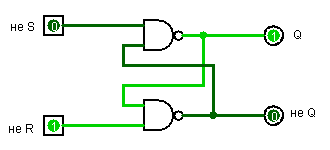
\includegraphics[width=0.8\textwidth]{1stepAsyncRSNAND.png}
		\caption{Реализация одноступенчатого асинхронного RS-триггера на элементах <<И-НЕ>>}
		\label{fig:1stepAsyncRSNAND}
	\end{figure}
	
\clearpage
\section{Одноступенчатый асинхронный RS-триггер на элементах <<ИЛИ-НЕ>>}
	Таблица переходов триггера (табл. \ref{table:1stepAsyncRSNOR}) и его функциональная схема (рис. \ref{fig:1stepAsyncRSNOR}).

	\begin{table}[H]
		\centering
		\caption{Таблица переходов одноступенчатого асинхронного RS-триггера на элементах <<ИЛИ-НЕ>>}
		\label{table:1stepAsyncRSNOR}
		\begin{tabular}{c|c|c|c|c}
			$ \overline{S} $ & $ \overline{R} $ & $ Q(t+1) $ & $ \overline{Q(t+1)} $ & Режим \\
			\hline
			0 & 0 & $ Q(t) $ & $\overline{Q(t)}$ & Хранение \\
			\hline
			0 & 1 & 0 & 1 & Установка 0 \\
			\hline
			1 & 0 & 1 & 0 & Установка 1 \\
			\hline
			1 & 1 & 0 & 0 & Запрещенная комбинация
		\end{tabular}
	\end{table}
	
	\begin{figure}[H]
		\centering
		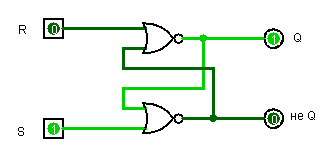
\includegraphics[width=0.8\textwidth]{1stepAsyncRSNOR.png}
		\caption{Реализация одноступенчатого асинхронного RS-триггера на элементах <<ИЛИ-НЕ>>}
		\label{fig:1stepAsyncRSNOR}
	\end{figure}

\clearpage
\section{Одноступенчатый синхронный RS-триггер на элементах <<И-НЕ>>}
	Таблица переходов триггера (табл. \ref{table:1stepSyncRSNAND}) и его функциональная схема (рис. \ref{fig:1stepSyncRSNAND}).

	\begin{table}[H]
		\centering
		\caption{Таблица переходов одноступенчатого синхронного RS-триггера на элементах <<И-НЕ>>}
		\label{table:1stepSyncRSNAND}
		\begin{tabular}{c|c|c|c|c|c}
			$ C $ & $ \overline{S} $ & $ \overline{R} $ & $ Q(t+1) $ & $ \overline{Q(t+1)} $ & Режим \\
			\hline
			0 & * & * & $ Q(t) $ & $\overline{Q(t)}$ & Хранение \\
			\hline
			1 & 0 & 0 & $ Q(t) $ & $\overline{Q(t)}$ & Хранение \\
			\hline
			1 & 0 & 1 & 0 & 1 & Установка 0 \\
			\hline
			1 & 1 & 0 & 1 & 0 & Установка 1 \\
			\hline
			1 & 1 & 1 & 1 & 1 & Запрещенная комбинация
		\end{tabular}
	\end{table}
	
	\begin{figure}[H]
		\centering
		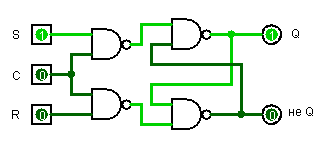
\includegraphics[width=0.8\textwidth]{1stepSyncRSNAND.png}
		\caption{Реализация одноступенчатого синхронного RS-триггера на элементах <<И-НЕ>>}
		\label{fig:1stepSyncRSNAND}
	\end{figure}

\clearpage
\section{Двухступенчатый синхронный RS-триггер с асинхронными входами предустановки, выполненный на элементах <<И-НЕ>>}
	Таблица переходов триггера (табл. \ref{table:2stepSyncRSNAND}) и его функциональная схема (рис. \ref{fig:2stepSyncRSNAND}).
	
	\begin{table}[H]
		\centering
		\caption{Таблица переходов двухступенчатого синхронного RS-триггера с асинхронными входами предустановки, выполненного на элементах <<И-НЕ>>}
		\label{table:2stepSyncRSNAND}
		\begin{tabular}{c|c|c|c|c|c|c|c}
			$ C $ & $ \overline{S} $ & $ \overline{R} $ & $ S $ & $ R $ & $ Q(t+1) $ & $ \overline{Q(t+1)} $ & Режим \\
			\hline
			* & 0 & 0 & * & * & 1 & 1 & Запрещенная комбинация \\
			\hline
			* & 0 & 1 & * & * & 1 & 0 & Асинхронная 1 \\
			\hline
			* & 1 & 0 & * & * & 0 & 1 & Асинхронный 0 \\
			\hline
			0 & 1 & 1 & * & * & $ Q(t) $ & $\overline{Q(t)}$ & Хранение \\
			\hline
			1 & 1 & 1 & * & * & $ Q(t) $ & $\overline{Q(t)}$ & Хранение \\
			\hline
			\texttiming{LH} & 1 & 1 & 0 & 1 & 0 & 1 & Синхронная установка 0 \\
			\hline
			\texttiming{LH} & 1 & 1 & 1 & 0 & 1 & 0 & Синхронная установка 1 \\
			\hline
			\texttiming{LH} & 1 & 1 & 1 & 1 & 1 & 1 & Запрещенная комбинация		
		\end{tabular}
	\end{table}
	
	\begin{figure}[H]
		\centering
		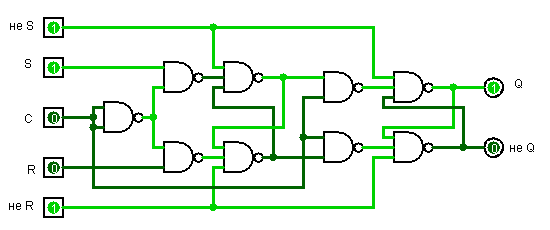
\includegraphics[width=\textwidth]{2stepSyncRSNAND.png}
		\caption{Реализация двухступенчатого синхронного RS-триггера с асинхронными входами предустановки, выполненного на элементах <<И-НЕ>>}
		\label{fig:2stepSyncRSNAND}
	\end{figure}

\clearpage
\section{Одноступенчатый D-триггер, выполненный на элементах <<И-НЕ>>}
	Таблица переходов триггера (табл. \ref{table:1stepDNAND}) и его функциональная схема (рис. \ref{fig:1stepDNAND}).
	
	\begin{table}[H]
		\centering
		\caption{Таблица переходов одноступенчатого D-триггера, выполненного на элементах <<И-НЕ>>}
		\label{table:1stepDNAND}
		\begin{tabular}{c|c|c|c|c}
			$ C $ & $ D $ & $ Q(t+1) $ & $ \overline{Q(t+1)} $ & Режим \\
			\hline
			0 & * & $ Q(t) $ & $ \overline{Q(t)} $ & Хранение \\
			\hline
			1 & 0 & 0 & 1 & Установка 0 \\
			\hline
			1 & 1 & 1 & 0 & Установка 1
		\end{tabular}
	\end{table}
	
	\begin{figure}[H]
		\centering
		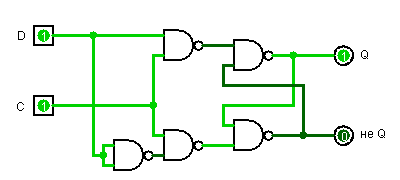
\includegraphics[width=0.8\textwidth]{1stepDNAND.png}
		\caption{Реализация одноступенчатого D-триггера, выполненного на элементах <<И-НЕ>>}
		\label{fig:1stepDNAND}
	\end{figure}

\clearpage	
\section{Динамический RS-триггер, работающий по переднему фронту, выполненный на элементах <<И-НЕ>>}
	Таблица переходов триггера (табл. \ref{table:DynRSNAND}) и его функциональная схема (рис. \ref{fig:DynRSNAND}).
	
	\begin{table}[H]
		\centering
		\caption{Таблица переходов динамического RS-триггера, работающего по переднему фронту, выполненного на элементах <<И-НЕ>>}
		\label{table:DynRSNAND}
		\begin{tabular}{c|c|c|c|c|c}
			$ C $ & $ \overline{S} $ & $ \overline{R} $ & $ Q(t+1) $ & $ \overline{Q(t+1)} $ & Режим \\
			\hline
			0 & * & * & $ Q(t) $ & $ \overline{Q(t)} $ & Хранение \\
			\hline
			1 & * & * & $ Q(t) $ & $ \overline{Q(t)} $ & Хранение \\
			\hline
			\texttiming{LH} & 0 & 0 & 0 & 0 & Запрещенная комбинация \\
			\hline
			\texttiming{LH} & 0 & 1 & 1 & 0 & Синхронная установка 1 \\
			\hline
			\texttiming{LH} & 1 & 0 & 0 & 1 & Синхронная установка 0 \\
			\hline
			* & 1 & 1 &	$ Q(t) $ & $ \overline{Q(t)} $ & Хранение
		\end{tabular}
	\end{table}
	
	\begin{figure}[H]
		\centering
		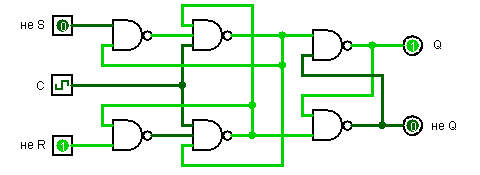
\includegraphics[width=\textwidth]{DynRSNAND.png}
		\caption{Реализация динамического RS-триггера, работающего по переднему фронту, выполненного на элементах <<И-НЕ>>}
		\label{fig:DynRSNAND}
	\end{figure}

\clearpage	
\section{Динамический RS-триггер, работающий по заднему фронту, выполненный на элементах <<ИЛИ-НЕ>>}
	Таблица переходов триггера (табл. \ref{table:DynRSNOR}) и его функциональная схема (рис. \ref{fig:DynRSNOR}).
	
	\begin{table}[H]
		\centering
		\caption{Таблица переходов динамического RS-триггера, работающего по заднему фронту, выполненного на элементах <<ИЛИ-НЕ>>}
		\label{table:DynRSNOR}
		\begin{tabular}{c|c|c|c|c|c}
			$ C $ & $ \overline{S} $ & $ \overline{R} $ & $ Q(t+1) $ & $ \overline{Q(t+1)} $ & Режим \\
			\hline
			0 & * & * & $ Q(t) $ & $ \overline{Q(t)} $ & Хранение \\
			\hline
			1 & * & * & $ Q(t) $ & $ \overline{Q(t)} $ & Хранение \\
			\hline
			\texttiming{HL} & 1 & 1 & 1 & 1 & Запрещенная комбинация \\
			\hline
			\texttiming{HL} & 0 & 1 & 1 & 0 & Синхронная установка 1 \\
			\hline
			\texttiming{HL} & 1 & 0 & 0 & 1 & Синхронная установка 0 \\
			\hline
			* & 0 & 0 &	$ Q(t) $ & $ \overline{Q(t)} $ & Хранение
		\end{tabular}
	\end{table}
	
	\begin{figure}[H]
		\centering
		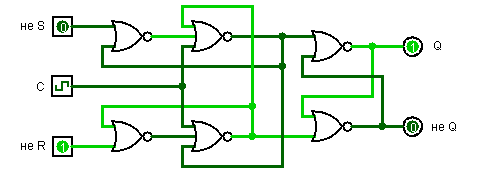
\includegraphics[width=\textwidth]{DynRSNOR.png}
		\caption{Реализация динамического RS-триггера, работающего по заднему фронту, выполненного на элементах <<ИЛИ-НЕ>>}
		\label{fig:DynRSNOR}
	\end{figure}

\clearpage	
\section{Т-триггер с асинхронными входами предустановки, выполненный на основе двухступенчатого RS-триггера}
	Таблица переходов триггера (табл. \ref{table:Ttrigger}) и его функциональная схема (рис. \ref{fig:Ttrigger}).
	
	\begin{table}[H]
		\centering
		\caption{Таблица переходов T-триггера с асинхронными входами предустановки, выполненного на основе двухступенчатого RS-триггера}
		\label{table:Ttrigger}
		\begin{tabular}{c|c|c|c|c|c}
			$ T $ & $ \overline{S} $ & $ \overline{R} $ & $ Q(t+1) $ & $ \overline{Q(t+1)} $ & Режим \\
			\hline
			* & 0 & 0 & 1 & 1 & Запрещенная комбинация \\
			\hline
			* & 0 & 1 & 1 & 0 & Асинхронная 1 \\
			\hline
			* & 1 & 0 & 0 & 1 & Асинхронный 0 \\
			\hline
			0 & 1 & 1 & $ Q(t) $ & $ \overline{Q(t)} $ & Хранение \\
			\hline
			1 & 1 & 1 & $ Q(t) $ & $ \overline{Q(t)} $ & Хранение \\
			\hline
			\texttiming{LH} & 1 & 1 & $ \overline{Q(t)} $ & $ Q(t) $ & Переключение в противоположное состояние
		\end{tabular}
	\end{table}
	
	\begin{figure}[H]
		\centering
		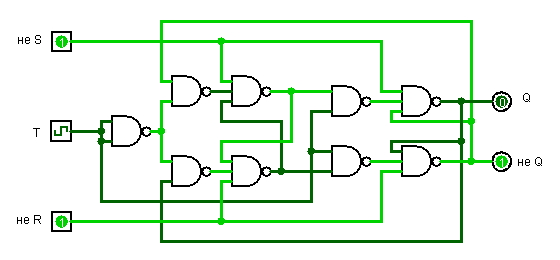
\includegraphics[width=\textwidth]{Ttrigger.png}
		\caption{Реализация T-триггера с асинхронными входами предустановки, выполненного на основе двухступенчатого RS-триггера}
		\label{fig:Ttrigger}
	\end{figure}

\clearpage	
\section{JK-триггер}
	Таблица переходов триггера (табл. \ref{table:JKtrigger}) и его функциональная схема (рис. \ref{fig:JKtrigger}).
		
	\begin{table}[H]
		\centering
		\caption{Таблица переходов JK-триггера, выполненного по схеме без инвертора}
		\label{table:JKtrigger}
		\begin{tabular}{c|c|c|c|c|c|c|c}
			$ C $ & $ \overline{S} $ & $ \overline{R} $ & $ J $ & $ K $ & $ Q(t+1) $ & $ \overline{Q(t+1)} $ & Режим \\
			\hline
			* & 0 & 0 & * & * & 1 & 1 & Запрещенная комбинация \\
			\hline
			* & 0 & 1 & * & * & 1 & 0 & Асинхронная 1 \\
			\hline
			* & 1 & 0 & * & * & 0 & 1 & Асинхронный 0 \\
			\hline
			0 & 1 & 1 & * & * & $ Q(t) $ & $\overline{Q(t)}$ & Хранение \\
			\hline
			1 & 1 & 1 & 1 & \texttiming{HL} & 0 & 1 & Подмена входов С и К \\
			\hline
			1 & 1 & 1 & \texttiming{HL} & 1 & 1 & 1 & Подмена входов С и R \\
			\hline
			\texttiming{HL} & 1 & 1 & 0 & 1 & 0 & 1 & Синхронная установка 0 \\
			\hline
			\texttiming{HL} & 1 & 1 & 1 & 0 & 1 & 0 & Синхронная установка 1 \\
			\hline
			\texttiming{HL} & 1 & 1 & 1 & 1 & 1 & 1 & Режим Т-триггера			
		\end{tabular}
	\end{table}
	
	\begin{figure}[H]
		\centering
		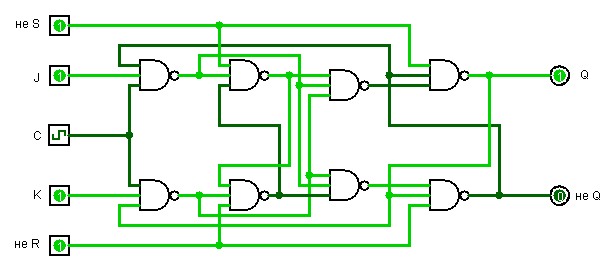
\includegraphics[width=\textwidth]{JKtrigger.png}
		\caption{Реализация JK-триггера, выполненного по схеме без инвертора}
		\label{fig:JKtrigger}
	\end{figure}

\chapter{ВЫВОДЫ}
В ходе работы были построены таблицы переходов триггеров и их схемы. После реализации схемы были протестированы, что позволило изучить принципы работы разного вида триггеров.
	
\begin{thebibliography}{99}
	\bibitem{Методичка} \textbf{Смирнов, С. С.} Информатика. Методические указания по выполнению практических работ / С. С. Смирнов, Д. А. Карпов. – Москва, МИРЭА – Российский технологический университет, 2020. – 102 с.
	
	\bibitem{Logisim} \textbf{Берч, К.} / Logisim : среда проектирования логических схем. -- версия 2.7.0. -- [б. м.], 2014. -- URL: http://www.cburch.com/logisim/index.html (дата обращения 26.10.2022). -- Электронная программа : электронная.
\end{thebibliography}
	
\end{document}
